\iffalse
\chapter{2015}
\author{AI24BTECH11028}
\section{st}
\fi


    \item \label{q1}  Rajiv Gandhi khel ratna award was conferred \underline{\hspace{2cm}}Mary kon, a six time world champion in boxing recently in a ceremony \underline{\hspace{2cm}} the Rashtrapati Bhawan(the president's official residence) in new delhi.
    \begin{enumerate}
        \item with, at
        \item on, in
        \item on, at
        \item to, at
    \end{enumerate}

    \item Despite a strinf of poor performances, the chances of K.L Rahul's selection in the team are\underline{\hspace{2cm}}
    \begin{enumerate}
        \item slim
        \item bright
        \item obvious
        \item uncertain
    \end{enumerate}

    \item Select the word that fites the analogy:
    Cover: Uncover :: Associate: \underline{\hspace{2cm}}
    \begin{enumerate}
        \item Unassociated
        \item Inassociate
        \item Misassociate
        \item Dissociate
    \end{enumerate}

    \item Hit by floods, the kharif(summer sown) crops in various parts of the country have been affected. Officials believe that the loss in production of the kharif crops can be recovered in the output of the rabi(winter sown) crops so that the country can achieve its food-grain production target of 291 million tons in the crop year 2019-20 (July- June). They are hopeful that good rains in July-August will help the soil retain moisture for a longer period, helping winter sown crops such as wheat and pulses during the November- February period.

    Which of the following statements can be inferred from the given passage?
    \begin{enumerate}
        \item Officials declared that the food-grain production target will be met due to good rains.
        \item Officials want the food grain production target to be met by the November-February period
        \item Officials feel that the food-grain production target cannot be met due to floods.
        \item Officials hope that the food-grain production target will be met due to good rabi produce.
    \end{enumerate}

    \item \label{q5}The difference between the sum of the first $2n$ natural numbers and the sum of the first $n$ odd natural numbers is\underline{\hspace{2cm}}
    \begin{enumerate}
        \item $n^2 - n$
        \item $n^2 + n$
        \item $2n^2 - n$
        \item $2n^2 + n$
    \end{enumerate}

\textbf{Q.\ref{q6} - Q.\ref{q10} carry two mark each}

\item \label{q6}Repo rate is the rate at which Reserve bank of India lends commercial banks, and reverse repo rate is the rate at which RBI borrows money from the commercial banks.

Which of the following statements can be inferred from the above passage?
\begin{enumerate}
    \item Decrease in repo rate will increase cost of borrowing and decrease lending by commercial banks.
    \item Increase in repo rate will decrease cost of borrowing and increase lending by commercial banks
    \item Increase in repo rate will decrease cost of borrowing and decrease lending by commercial banks
    \item Decrease in repo rate will decrease cost of borrowing and increase lending by commercial banks
\end{enumerate}

\item P, Q, R, S, T, U, V and W are seated around at circular table.\\
    I. S is seated opposite to W. \\
    II. U is seated at the second place to the right of R.\\
    III. T is seated at the third place to left of R.\\
    IV. V is a neighbour of S.\\
Which of the following must be true?
\begin{enumerate}
    \item P is the neighbour of R
    \item Q is a neighbour of R
    \item P is not seated opposite to Q
    \item R is the left neighbour of S
\end{enumerate}

\item The distance between Delhi and Agra is 233km.A car P started travelling from Deli to Agra and another car Q started from Agra to Delhi along the same road 1 hours after the car P started. The two cars crossed each other 75 minutes after the car Q is started. Both cars were travelling at constant speed. The spped of ar P was 10km/hr more than the speed of car Q. How many kilometer the car Q had travelled when the cars crossed each other?
\begin{enumerate}
    \item 66.6
    \item 75.2
    \item 88.2
    \item 116.5
\end{enumerate}

\item For matrix $M = [m_{ij}]; i,j = 1,2,3,4$ the diagonal elements are all zero and $m_{ij} = -m_{ji}$. The minimum number of elements required to fully specify the matrix is \underline{\hspace{2cm}}
\begin{enumerate}
    \item 0
    \item 6
    \item 12
    \item 16
\end{enumerate}

\item \label{q10} The profit shares of two companies P and Q are shown in the figure. If the two companies have invested a fixed and equal amount every year, then the ratio of the total revenue of the company P to the total revenue of company Q, during 2013-2018 is \underline{\hspace{2cm}}
\begin{figure}[h!]
    \centering
    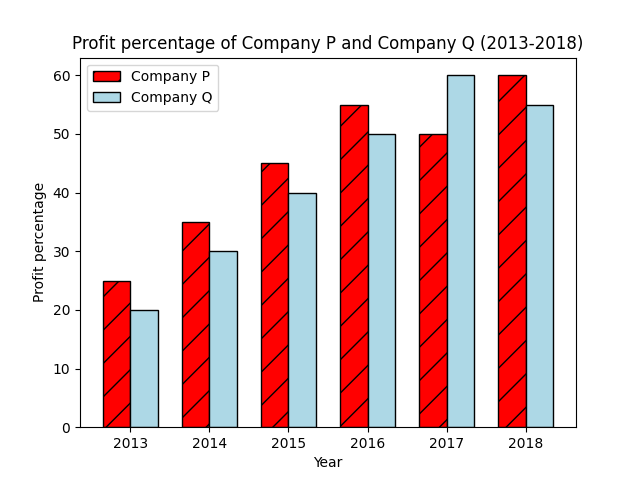
\includegraphics[width=0.5\linewidth]{figs/ST-2015/ST-2022.png} 
\end{figure}
\begin{enumerate}
    \item 15 : 17
    \item 16 : 17
    \item 17 : 15
    \item 17: 16
\end{enumerate}


\textbf{Q.\ref{q11} - Q.\ref{q35} carry one mark each}
\item \label{q11}
    Let $M$ be a $3 \times 3$ non-zero idempotent matrix and let $I_3$ denote the $3 \times 3$ identity matrix. Then which of the following statements is \textbf{FALSE}?
\begin{enumerate}
    \item The eigenvalues of $M$ are $0$ and $1$.
    \item $\text{Rank}(M) = \text{Trace}(M)$.
    \item $I_3 - M$ is idempotent.
    \item $(I_3 + M)^{-1} = I_3 - 2M$.
\end{enumerate}

\item
Let $\mathbb{C}$ denote the set of all complex numbers. Consider the vector space
\[
V = \{(a, b, c) : a, b, c \in \mathbb{C} ;  a + \overline{b} = 0 ;  b + \overline{c} = 0 \},
\]
over the field of real numbers, where for any complex number $z$, $\overline{z}$ denotes its complex conjugate. If $i = \sqrt{-1}$, then a basis of $V$ is
\begin{enumerate}
    \item $\{\brak{1, -1, 1}, \brak{i, i, i}\}$
    \item $\{\brak{1, -1, 1}, \brak{i, -i, i}\}$
    \item $\{\brak{1, -i, 1}, \brak{i, 1, i}\}$
    \item $\{\brak{1, -i, 1}, \brak{i, 1, -i}\}$
\end{enumerate}

\item 
Let $S = \{(x, y) \in \mathbb{R} \times \mathbb{R} : x^2 - y^2 = 4\}$ and $f: S \rightarrow \mathbb{R}$ be defined by
\[
f(x, y) = 6x + y^2,
\]
where $\mathbb{R}$ denotes the set of all real numbers. Then
\begin{enumerate}
    \item $f$ is bounded on $S$.
    \item the maximum value of $f$ on $S$ is 13.
    \item the minimum value of $f$ on $S$ is -14.
    \item the minimum value of $f$ on $S$ is -13.
\end{enumerate}


